\section{Resultados}\label{sec:resultados}

Los resultados se presentan en el orden de los objetivos específicos. Las cifras de
validación cruzada corresponden a \textit{dev} y las del conjunto de prueba sellado, a su
única evaluación.

\subsection{Caracterización de los datos (objetivo específico 1)}\label{sec:res-eda}

El hallazgo central del análisis exploratorio es que la tasa de fraude depende de cuánto
historial tiene el cliente. Entre el decil con menos facturas (1 a 3) y el decil con más (70
a 439) la tasa pasa de 0,642\,\% a 9,756\,\%, un factor de 15,2
(Figura~\ref{fig:historial}). Un historial largo da más ocasiones de inspección, de modo que
parte de lo que un modelo aprendería como señal es exposición acumulada. El número de
contadores del cliente tenía el mayor tamaño de efecto de todas las variables exploratorias
(rango-biserial 0,415) y lo conserva entre 0,22 y 0,40 dentro de cada quintil de longitud
del historial. El índice máximo acumulado, en cambio, cae a $-0{,}015$ en el quintil de
historial más largo: medía exposición y no comportamiento.

\begin{figure}[htbp]
  \centering
  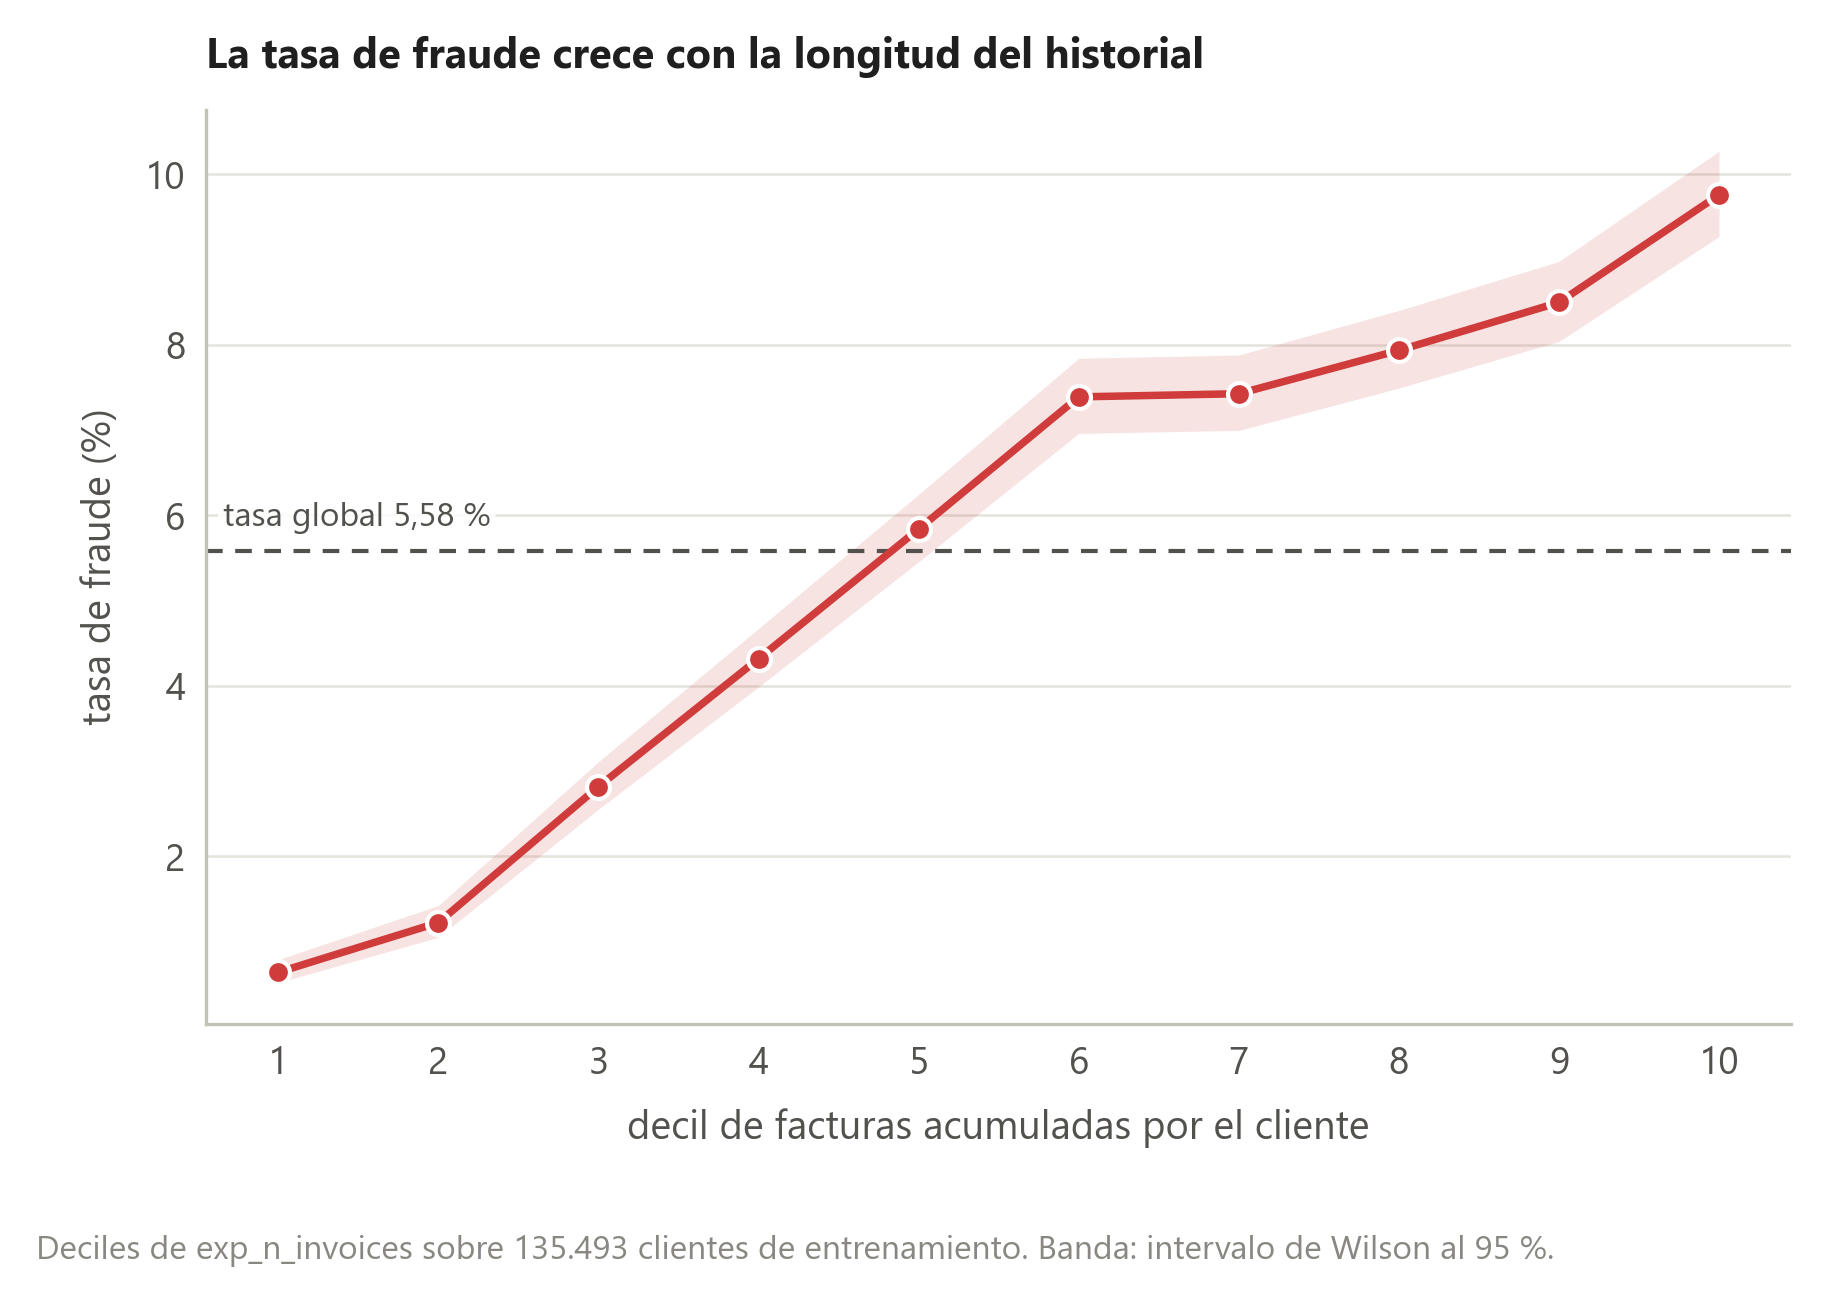
\includegraphics[width=0.72\textwidth]{fig_confusion_historial.png}
  \caption{Tasa de fraude por decil de número de facturas del cliente, con intervalo de
    Wilson al 95\,\%, sobre los 135.493 clientes de entrenamiento.}
  \label{fig:historial}
\end{figure}

El desbalance es marcado pero no hay escasez de casos: 5,58\,\% de positivos, con unos 1.200
positivos en cada pliegue de validación de \textit{dev}. La tasa de fraude también crece con
el consumo máximo del cliente, del 0,649\,\% en el decil más bajo al 11,446\,\% en el más
alto, lo que respalda la decisión de no recortar los consumos extremos.

La Figura~\ref{fig:calidad} resume las anomalías de captura de las facturas. La más
frecuente es el consumo total igual a cero, en el 10,4\,\% de las facturas, seguida de
números de contador iguales a cero y de duplicados por clave lógica. Ninguna afecta a más
del 1\,\% de las filas salvo la primera, y ninguna obligó a descartar clientes. La partición
original de Zindi entre entrenamiento y prueba es aleatoria por cliente: el año de la última
factura se distribuye igual en ambos archivos (V de Cramér corregida 0,003, $p = 0{,}32$).

\begin{figure}[htbp]
  \centering
  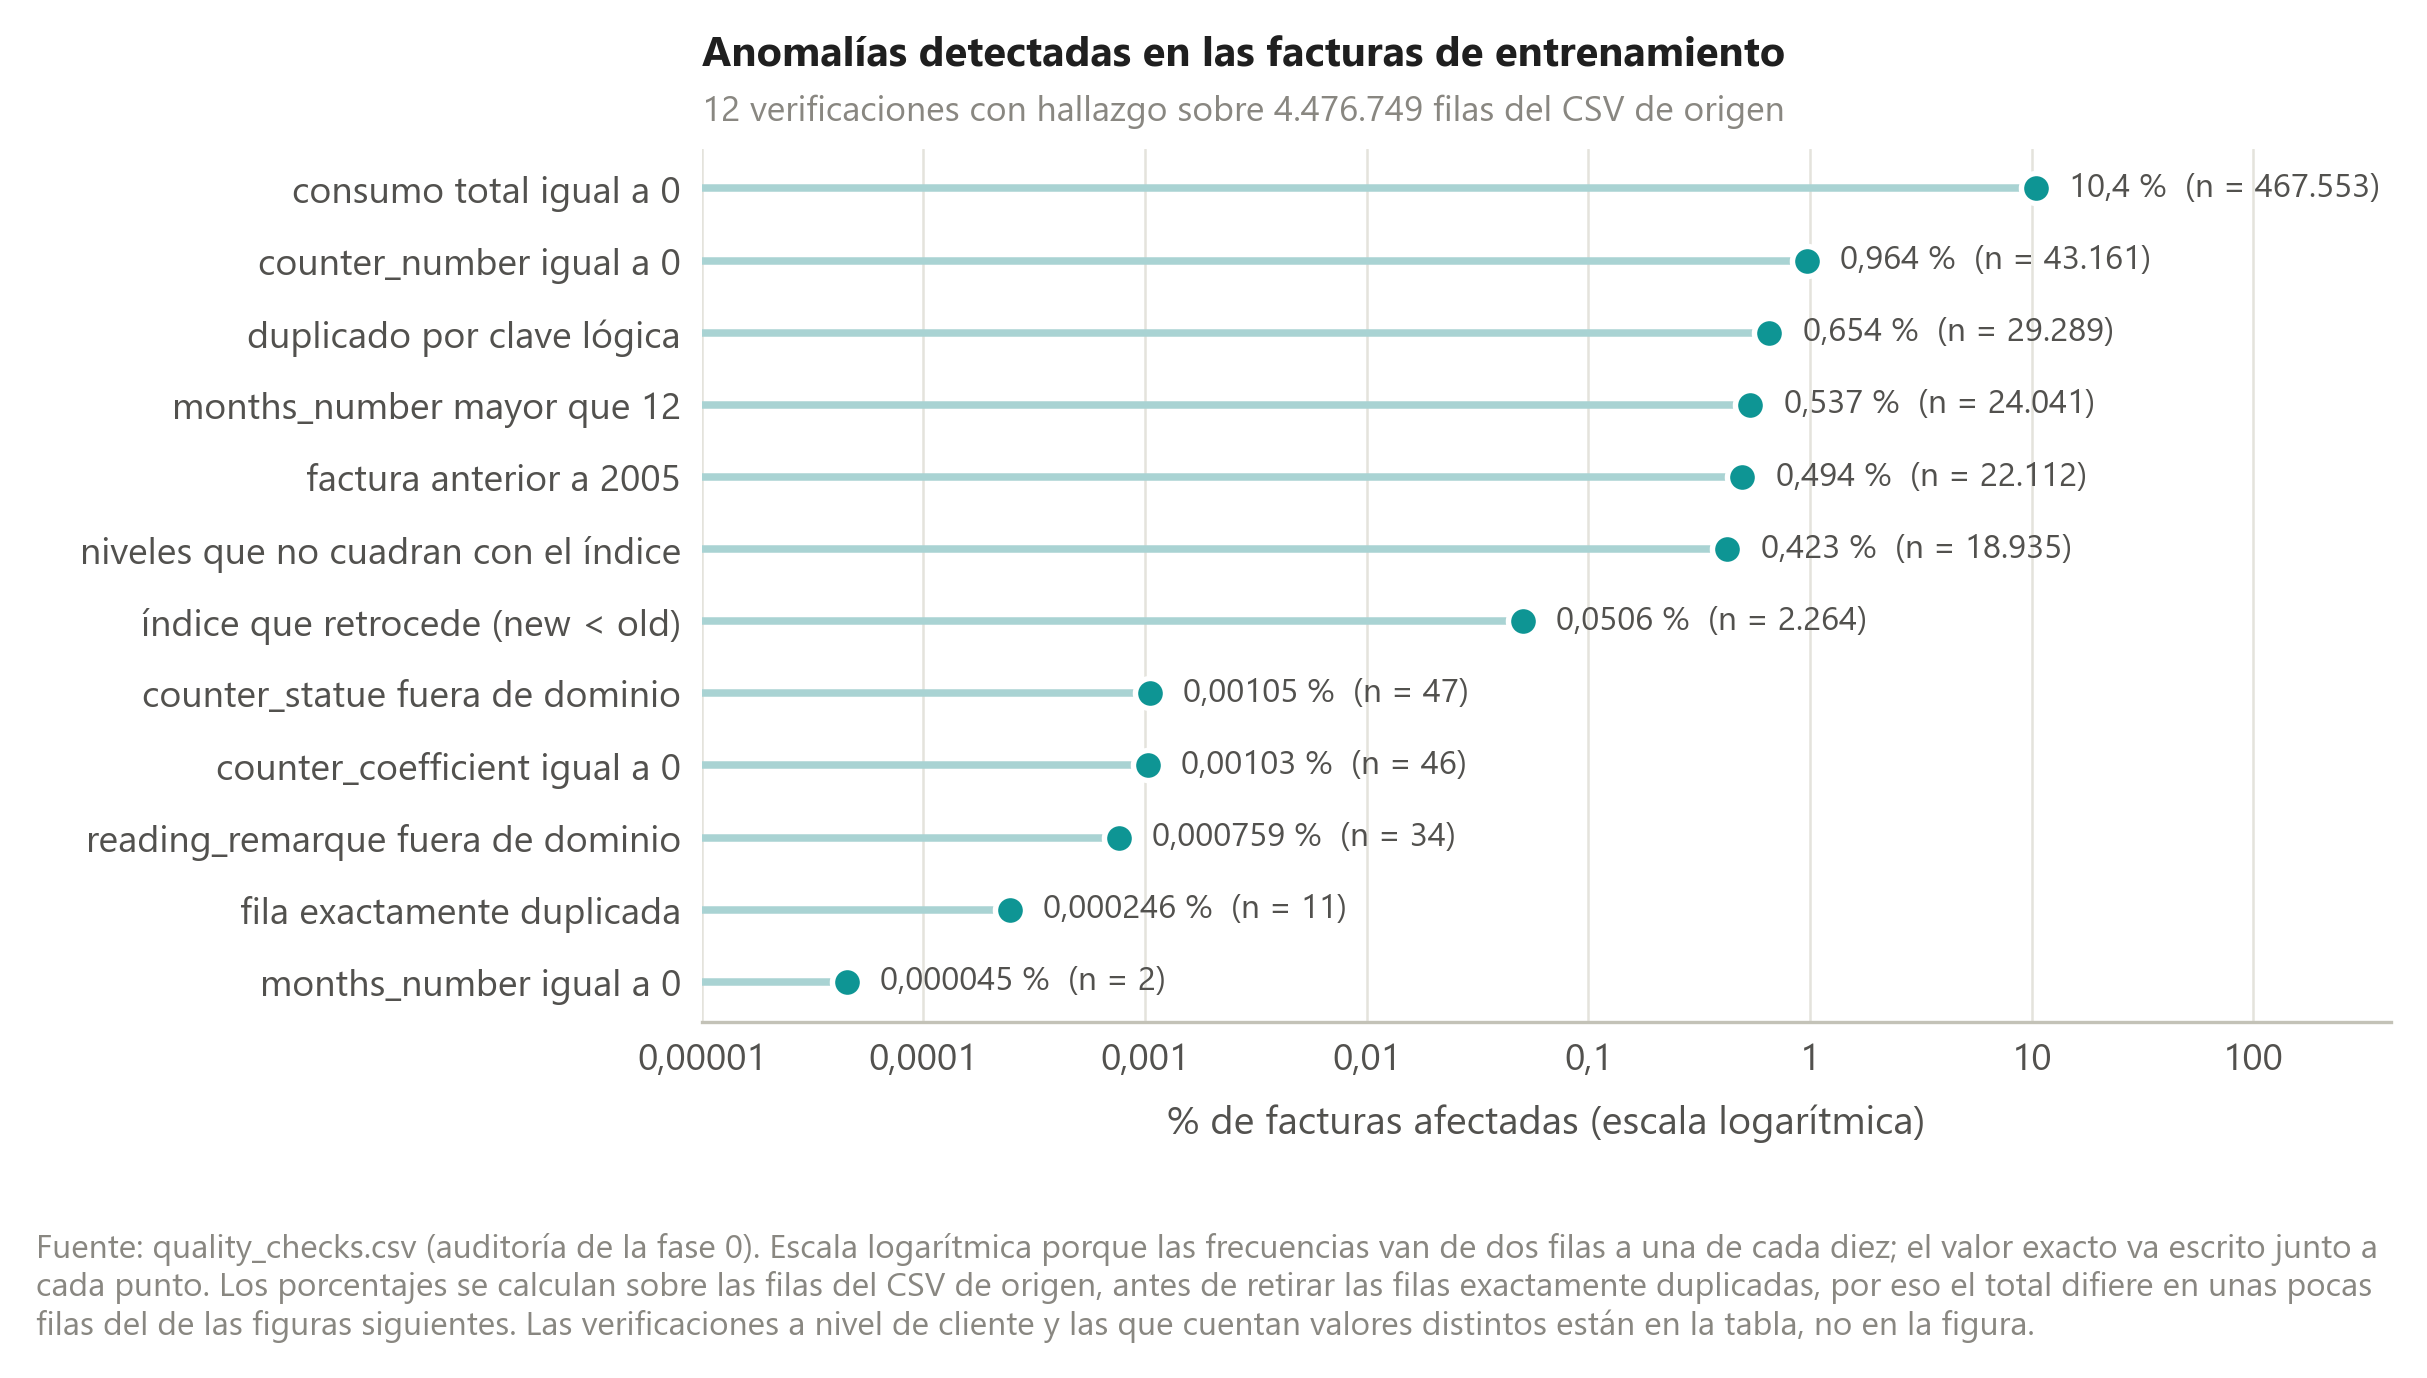
\includegraphics[width=0.9\textwidth]{fig_calidad_anomalias.png}
  \caption{Porcentaje de facturas de entrenamiento afectadas por cada anomalía detectada en
    la auditoría de calidad, en escala logarítmica.}
  \label{fig:calidad}
\end{figure}

\subsection{Variables y comparación de modelos (objetivo específico 2)}

\subsubsection{Huellas de la inspección en el historial}\label{sec:res-huellas}

Los eventos de equipo y de contrato se comportan como consecuencia de la inspección
(Tabla~\ref{tab:eventos}). Los 22.217 clientes de \textit{dev} con alguno de ellos tienen una
tasa de fraude del 18,7\,\%, frente al 2,2\,\% del resto. En los clientes con fraude, el
reemplazo del contador ocurre hacia el final del historial, con una posición relativa
mediana de 0,70 frente a 0,41 en los demás, y después del último reemplazo les quedan 2,7
años de historial frente a 5,7. El código de contador 207 pasa del 7,4\,\% al 10,8\,\% de las
facturas entre la primera y la segunda mitad del historial, y solo en los clientes con
fraude, lo que es compatible con la instalación de un equipo nuevo tras la inspección.

% Generado por paper/exportar_artefactos.py desde reports/tables/modeling_diagnostico_eventos_equipo.csv. No editar a mano.
\begin{table}[htbp]
  \centering
  \small
  \caption{Eventos de equipo y de contrato en el historial de los clientes de \textit{dev}.}
  \label{tab:eventos}
  \begin{threeparttable}
    \begin{tabular}{l S[table-format=5.0] S[table-format=2.1] S[table-format=1.1] S[table-format=1.2] S[table-format=1.2]}
      \toprule
      {Evento} & {Clientes} & {\shortstack{Fraude con\\evento (\%)}} & {\shortstack{Fraude sin\\evento (\%)}} & {\shortstack{Posición\\(fraude)}} & {\shortstack{Posición\\(sin fraude)}} \\
      \midrule
      Reemplazo de contador & 19163 & 18.1 & 2.9 & 0.70 & 0.41 \\
      Cambio de código de contador & 4285 & 26.9 & 4.7 & 0.69 & 0.52 \\
      Cambio de tarifa & 1612 & 17.2 & 5.4 & 0.59 & 0.60 \\
      Cualquiera de los tres & 22217 & 18.7 & 2.2 & 0.69 & 0.47 \\
      \bottomrule
    \end{tabular}
    \begin{tablenotes}
      \footnotesize
      \item Posición: ubicación relativa mediana del evento dentro del historial del cliente (0 = primera factura, 1 = última).
      \item Fuente: \texttt{reports/tables/modeling\_diagnostico\_eventos\_equipo.csv}.
    \end{tablenotes}
  \end{threeparttable}
\end{table}


La verificación por mitades confirma H1 (Tabla~\ref{tab:mitades}). Con el historial
completo, las variables de la segunda mitad alcanzan un PR-AUC de 0,396 y las de la primera
0,182, una diferencia de 0,213 (IC 95\,\% [0,199; 0,227]). Con el historial censurado la
diferencia baja a 0,032 (IC 95\,\% [0,022; 0,041]). La tasa de cambio de contador aporta por
sí sola 0,10 de PR-AUC al modelo con historial completo (0,363 frente a 0,260 sin ella).

% Generado por paper/exportar_artefactos.py desde reports/tables/modeling_verificacion_mitades_historial.csv. No editar a mano.
\begin{table}[htbp]
  \centering
  \small
  \caption{Verificación por mitades del historial: PR-AUC en validación cruzada sobre \textit{dev} con variables calculadas en cada mitad.}
  \label{tab:mitades}
  \begin{threeparttable}
    \begin{tabular}{l l S[table-format=5.0] S[table-format=1.3] c c}
      \toprule
      {Historial} & {Variables de} & {Clientes} & {PR-AUC} & {IC 95\,\%} & {Diferencia con la primera mitad} \\
      \midrule
      Completo & Primera mitad & 74109 & 0.182 & {[0,172; 0,189]} & {---} \\
      Completo & Segunda mitad & 74109 & 0.396 & {[0,381; 0,408]} & {0,213 [0,199; 0,227]} \\
      Completo & Historial entero & 74109 & 0.375 & {[0,362; 0,388]} & {0,194 [0,181; 0,206]} \\
      Censurado & Primera mitad & 64437 & 0.185 & {[0,173; 0,194]} & {---} \\
      Censurado & Segunda mitad & 64437 & 0.217 & {[0,204; 0,225]} & {0,032 [0,022; 0,041]} \\
      Censurado & Historial entero & 64437 & 0.226 & {[0,212; 0,235]} & {0,041 [0,032; 0,049]} \\
      \bottomrule
    \end{tabular}
    \begin{tablenotes}
      \footnotesize
      \item Clientes de \textit{dev} con al menos 16 facturas, para que cada mitad tenga 8 o más; se usan los mismos pliegues restringidos a esa población.
      \item Fuente: \texttt{reports/tables/modeling\_verificacion\_mitades\_historial.csv}.
    \end{tablenotes}
  \end{threeparttable}
\end{table}


\subsubsection{Comparación de modelos}

Con el historial censurado, LightGBM obtiene el mayor PR-AUC en validación cruzada, 0,192
con una desviación de 0,006 entre pliegues, y un ROC-AUC de 0,768 (Tabla~\ref{tab:modelos} y
Figura~\ref{fig:modelos}). XGBoost queda a una diferencia de $-0{,}002$ (IC 95\,\%
[$-0{,}004$; 0,001]) y es indistinguible; por la regla de selección se prefiere LightGBM con
hiperparámetros por defecto. La búsqueda con Optuna y la ponderación de clases dan valores
inferiores en los cinco pliegues, con intervalos que excluyen el cero, así que no se
adoptaron. La regresión logística se queda en 0,131, por debajo de los modelos de boosting y
apenas por encima de la línea base de exposición (0,124). La prevalencia, equivalente al
azar, marca 0,056.

% Generado por paper/exportar_artefactos.py desde reports/tables/model_comparison.csv. No editar a mano.
\begin{table}[htbp]
  \centering
  \small
  \caption{Comparación de modelos en validación cruzada de 5 pliegues sobre \textit{dev} (108.394 clientes, historial censurado).}
  \label{tab:modelos}
  \begin{threeparttable}
    \begin{tabular}{l S[table-format=1.3] S[table-format=1.3] S[table-format=1.3] c S[table-format=1.1]}
      \toprule
      {Modelo} & {PR-AUC} & {Desv.} & {ROC-AUC} & {Diferencia de PR-AUC [IC 95\,\%]} & {Lift@1\,\%} \\
      \midrule
      Prevalencia (azar) & 0.056 & 0.001 & 0.500 & {$-$0,135 [$-$0,145; $-$0,127]} & 1.0 \\
      Solo exposición & 0.124 & 0.005 & 0.732 & {$-$0,068 [$-$0,077; $-$0,060]} & 3.8 \\
      Regresión logística & 0.131 & 0.009 & 0.721 & {$-$0,062 [$-$0,069; $-$0,054]} & 4.3 \\
      XGBoost & 0.190 & 0.007 & 0.767 & {$-$0,002 [$-$0,004; 0,001]} & 6.9 \\
      LightGBM ponderado & 0.185 & 0.009 & 0.763 & {$-$0,007 [$-$0,010; $-$0,004]} & 6.9 \\
      LightGBM con Optuna & 0.187 & 0.008 & 0.766 & {$-$0,004 [$-$0,007; $-$0,001]} & 6.8 \\
      LightGBM (seleccionado) & 0.192 & 0.006 & 0.768 & {---} & 6.7 \\
      \bottomrule
    \end{tabular}
    \begin{tablenotes}
      \footnotesize
      \item PR-AUC y ROC-AUC: media de los 5 pliegues; Desv.: desviación estándar entre pliegues.
      \item Diferencia frente al modelo seleccionado sobre las predicciones fuera de pliegue, con IC por bootstrap pareado por cliente.
      \item Fuente: \texttt{reports/tables/model\_comparison.csv}.
    \end{tablenotes}
  \end{threeparttable}
\end{table}


\begin{figure}[htbp]
  \centering
  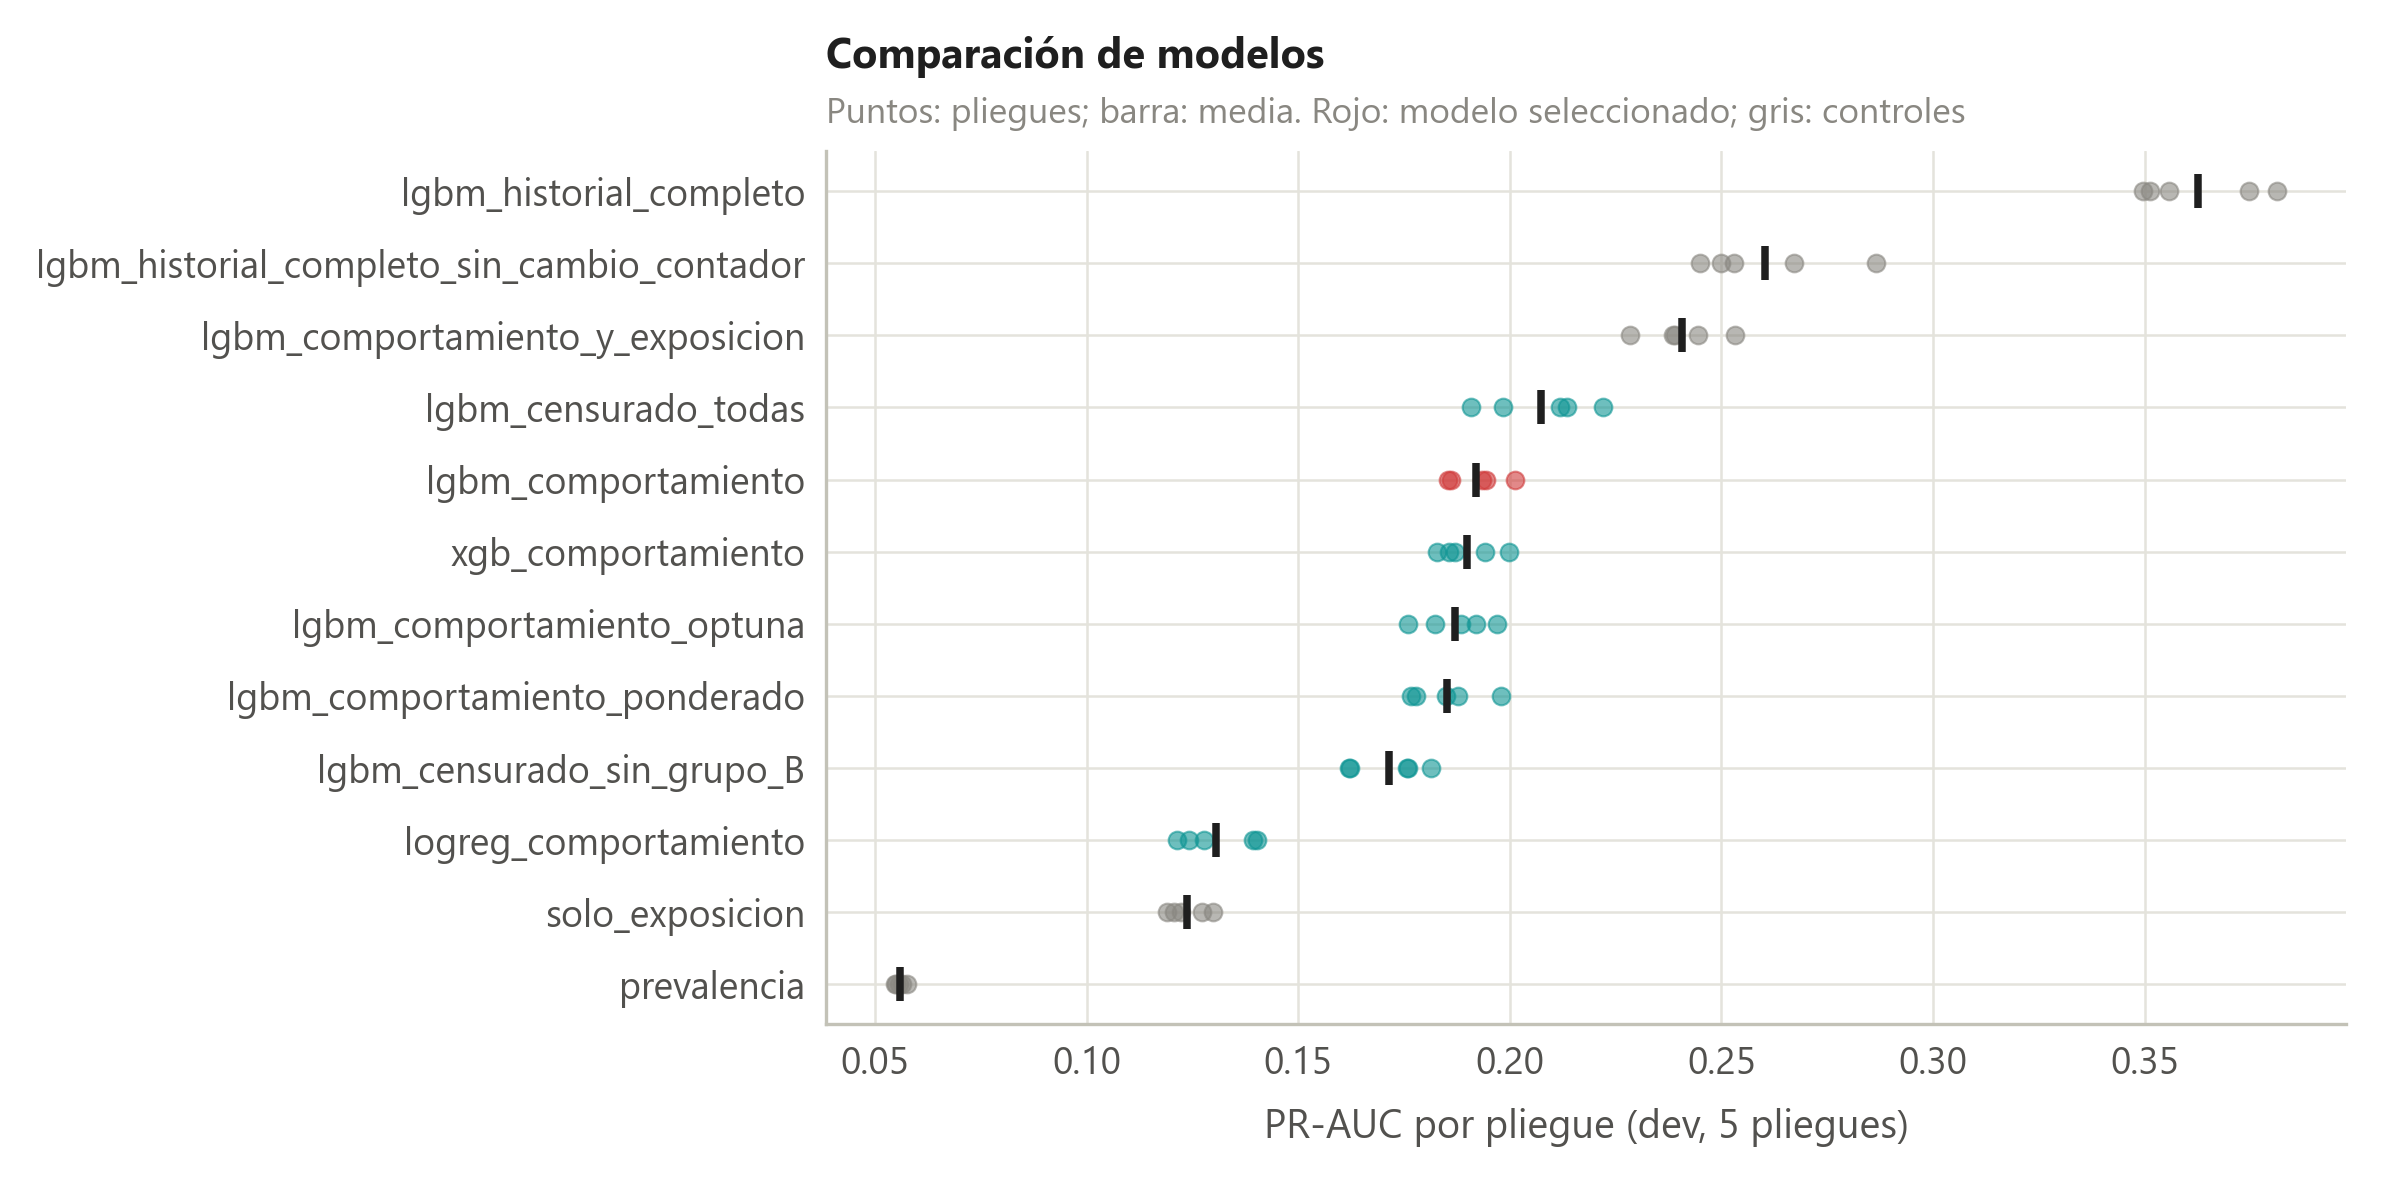
\includegraphics[width=\textwidth]{fig_model_comparacion_pr_auc.png}
  \caption{PR-AUC por pliegue de cada modelo en validación cruzada sobre \textit{dev}. La
    barra marca la media; en rojo el modelo seleccionado y en gris los controles.}
  \label{fig:modelos}
\end{figure}

Los controles muestran cuánto desempeño procede de fuentes que no son el comportamiento del
cliente. El mismo LightGBM con el historial completo llega a 0,363 de PR-AUC y con las
variables de exposición añadidas a 0,241. La puntuación del modelo seleccionado tiene una
correlación de Spearman de 0,42 con el número de facturas, frente a 0,688 de la línea base
de exposición. Dentro de cada quintil de longitud del historial, donde la exposición está
aproximadamente controlada, su ROC-AUC va de 0,707 a 0,775, mientras el de la línea base de
exposición cae de 0,868 en el quintil más corto a 0,632 en el más largo
(Figura~\ref{fig:quintiles}).

\begin{figure}[htbp]
  \centering
  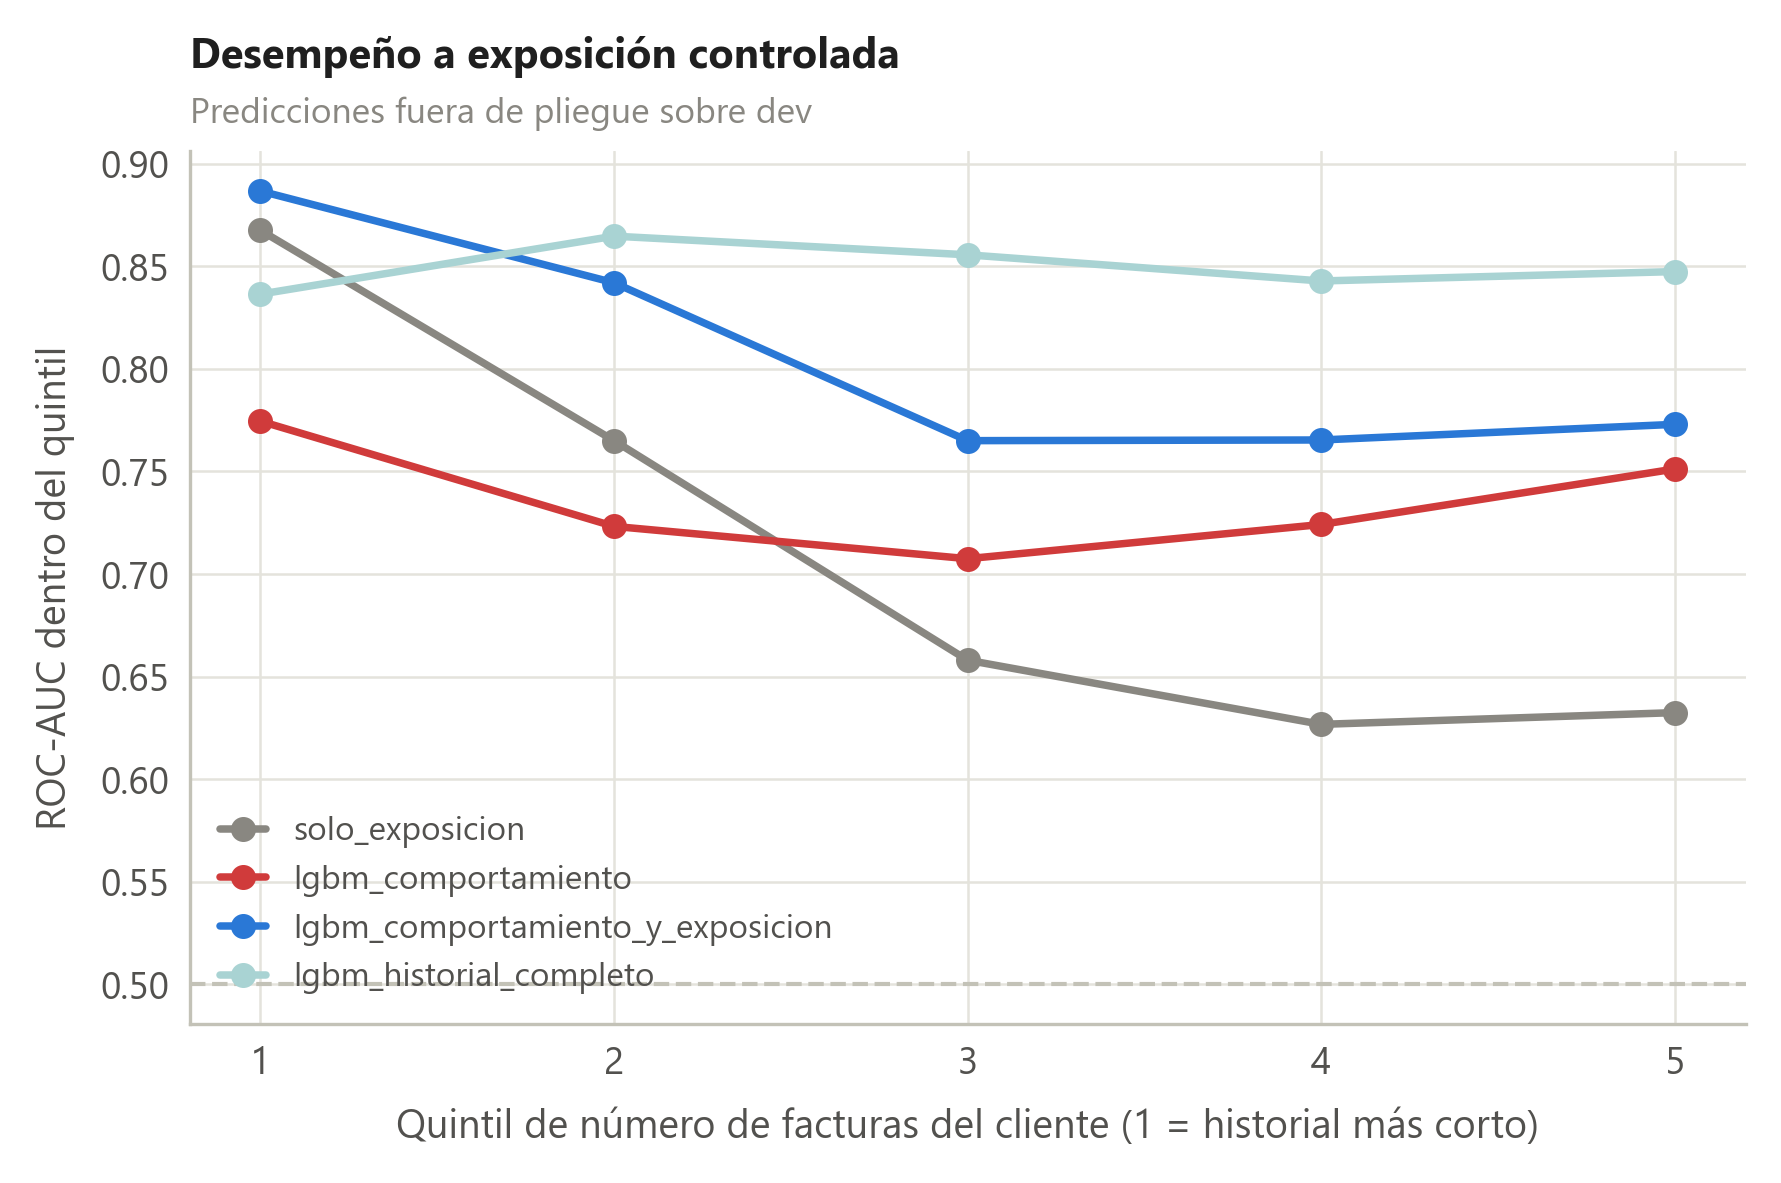
\includegraphics[width=0.75\textwidth]{fig_model_quintiles_historial.png}
  \caption{ROC-AUC dentro de cada quintil de número de facturas, con predicciones fuera de
    pliegue sobre \textit{dev}.}
  \label{fig:quintiles}
\end{figure}

En los 86.177 clientes de \textit{dev} sin ningún evento de equipo o de contrato, con una
prevalencia del 2,2\,\%, el modelo obtiene un ROC-AUC de 0,778 frente a 0,714 de la línea base
de exposición, y un PR-AUC de 0,098. Repetida con otras dos semillas de partición, la
validación cruzada da un PR-AUC medio entre 0,188 y 0,192.

\subsection{Evaluación práctica e interpretación (objetivo específico 3)}

\subsubsection{Desempeño en el conjunto de prueba sellado}

En su única evaluación sobre el conjunto de prueba, el modelo seleccionado obtiene un PR-AUC
de 0,191 (IC 95\,\% [0,174; 0,211]) y un ROC-AUC de 0,762 (IC 95\,\% [0,750; 0,773])
(Tabla~\ref{tab:holdout}). La cifra coincide con la de validación cruzada (0,192), así que el
proceso de selección no produjo un resultado optimista. Supera a la línea base de exposición
en 0,060 de PR-AUC (IC 95\,\% [0,042; 0,077]). El control de sensibilidad sin el grupo B de
variables queda en 0,174 (IC 95\,\% [0,158; 0,192]); aun sin ese grupo, el modelo sigue por
encima de la línea base de exposición, así que la conclusión principal no depende de él.

% Generado por paper/exportar_artefactos.py desde reports/tables/modeling_holdout_metricas.csv. No editar a mano.
\begin{table}[htbp]
  \centering
  \small
  \caption{Desempeño en el holdout sellado (27.099 clientes, 1.513 positivos), evaluado una sola vez.}
  \label{tab:holdout}
  \begin{threeparttable}
    \begin{tabular}{l S[table-format=1.3] c S[table-format=1.3] S[table-format=1.4] S[table-format=2.1] S[table-format=2.1]}
      \toprule
      {Modelo} & {PR-AUC} & {IC 95\,\%} & {ROC-AUC} & {Brier} & {Precisión@1\,\% (\%)} & {Lift@1\,\%} \\
      \midrule
      LightGBM (seleccionado) & 0.191 & {[0,174; 0,211]} & 0.762 & 0.0490 & 43.5 & 7.8 \\
      LightGBM sin grupo B & 0.174 & {[0,158; 0,192]} & 0.742 & 0.0497 & 36.9 & 6.6 \\
      Solo exposición & 0.132 & {[0,122; 0,144]} & 0.745 & 0.0506 & 21.0 & 3.8 \\
      LightGBM con exposición & 0.243 & {[0,223; 0,265]} & 0.818 & 0.0472 & 46.9 & 8.4 \\
      LightGBM historial completo & 0.381 & {[0,359; 0,407]} & 0.879 & 0.0418 & 60.1 & 10.8 \\
      \bottomrule
    \end{tabular}
    \begin{tablenotes}
      \footnotesize
      \item Las dos últimas filas son controles: la exposición mide oportunidades de inspección y el historial completo contiene huellas posteriores a la detección; no son candidatos.
      \item IC del PR-AUC por bootstrap de clientes (1.000 réplicas).
      \item Fuente: \texttt{reports/tables/modeling\_holdout\_metricas.csv}.
    \end{tablenotes}
  \end{threeparttable}
\end{table}


\subsubsection{Fraudes encontrados en una lista de tamaño fijo}

La Tabla~\ref{tab:curva-k} traduce el ordenamiento a campañas de inspección. Si la empresa
visita el 1\,\% de los clientes, 271 en el conjunto de prueba, el modelo encuentra 118 fraudes,
con una precisión del 43,5\,\%. La línea base de exposición encontraría 57 y una selección al
azar, 15. Es una precisión 7,8 veces mayor que la prevalencia y el doble que la de la línea
base. Con listas más largas la precisión baja, como es de esperar, y el lift pasa de 7,3 en el
0,5\,\% a 3,4 en el 10\,\%. Esa lista del 1\,\% recupera el 7,8\,\% de los fraudes, frente a un
techo del 17,9\,\% que impone su tamaño.

% Generado por paper/exportar_artefactos.py desde reports/tables/modeling_holdout_curva_k.csv y modeling_holdout_metricas.csv. No editar a mano.
\begin{table}[htbp]
  \centering
  \small
  \caption{Fraudes encontrados en el holdout según el tamaño de la lista de inspección.}
  \label{tab:curva-k}
  \begin{threeparttable}
    \begin{tabular}{l S[table-format=4.0] S[table-format=3.0] S[table-format=3.0] S[table-format=3.0] S[table-format=2.1] S[table-format=2.1] S[table-format=3.1]}
      \toprule
      {Lista} & {$k$} & {Azar} & {\shortstack{Regla de\\exposición}} & {Modelo} & {\shortstack{Precisión\\(\%)}} & {\shortstack{Recall\\(\%)}} & {\shortstack{Techo de\\recall (\%)}} \\
      \midrule
      0,5\,\% & 135 & 8 & 28 & 55 & 40.7 & 3.6 & 8.9 \\
      1,0\,\% & 271 & 15 & 57 & 118 & 43.5 & 7.8 & 17.9 \\
      2,0\,\% & 542 & 30 & 117 & 192 & 35.4 & 12.7 & 35.8 \\
      5,0\,\% & 1355 & 76 & 234 & 352 & 26.0 & 23.3 & 89.6 \\
      10,0\,\% & 2710 & 151 & 404 & 521 & 19.2 & 34.4 & 100.0 \\
      \bottomrule
    \end{tabular}
    \begin{tablenotes}
      \footnotesize
      \item Azar: prevalencia por $k$. Regla de exposición y modelo: precisión@$k$ por $k$. Precisión, recall y techo corresponden al modelo seleccionado.
      \item Techo de recall: $\min(k, P)/P$, con $P$ = 1.513 positivos del holdout.
      \item Fuente: \texttt{reports/tables/modeling\_holdout\_curva\_k.csv y modeling\_holdout\_metricas.csv}.
    \end{tablenotes}
  \end{threeparttable}
\end{table}


Las probabilidades están calibradas sin necesidad de ajuste (Figura~\ref{fig:holdout},
derecha): en el decil de menor puntuación la probabilidad media predicha es 0,0024 y la tasa
observada 0,0022, y en el decil superior, 0,203 frente a 0,192. La puntuación de Brier es
0,049.

\begin{figure}[htbp]
  \centering
  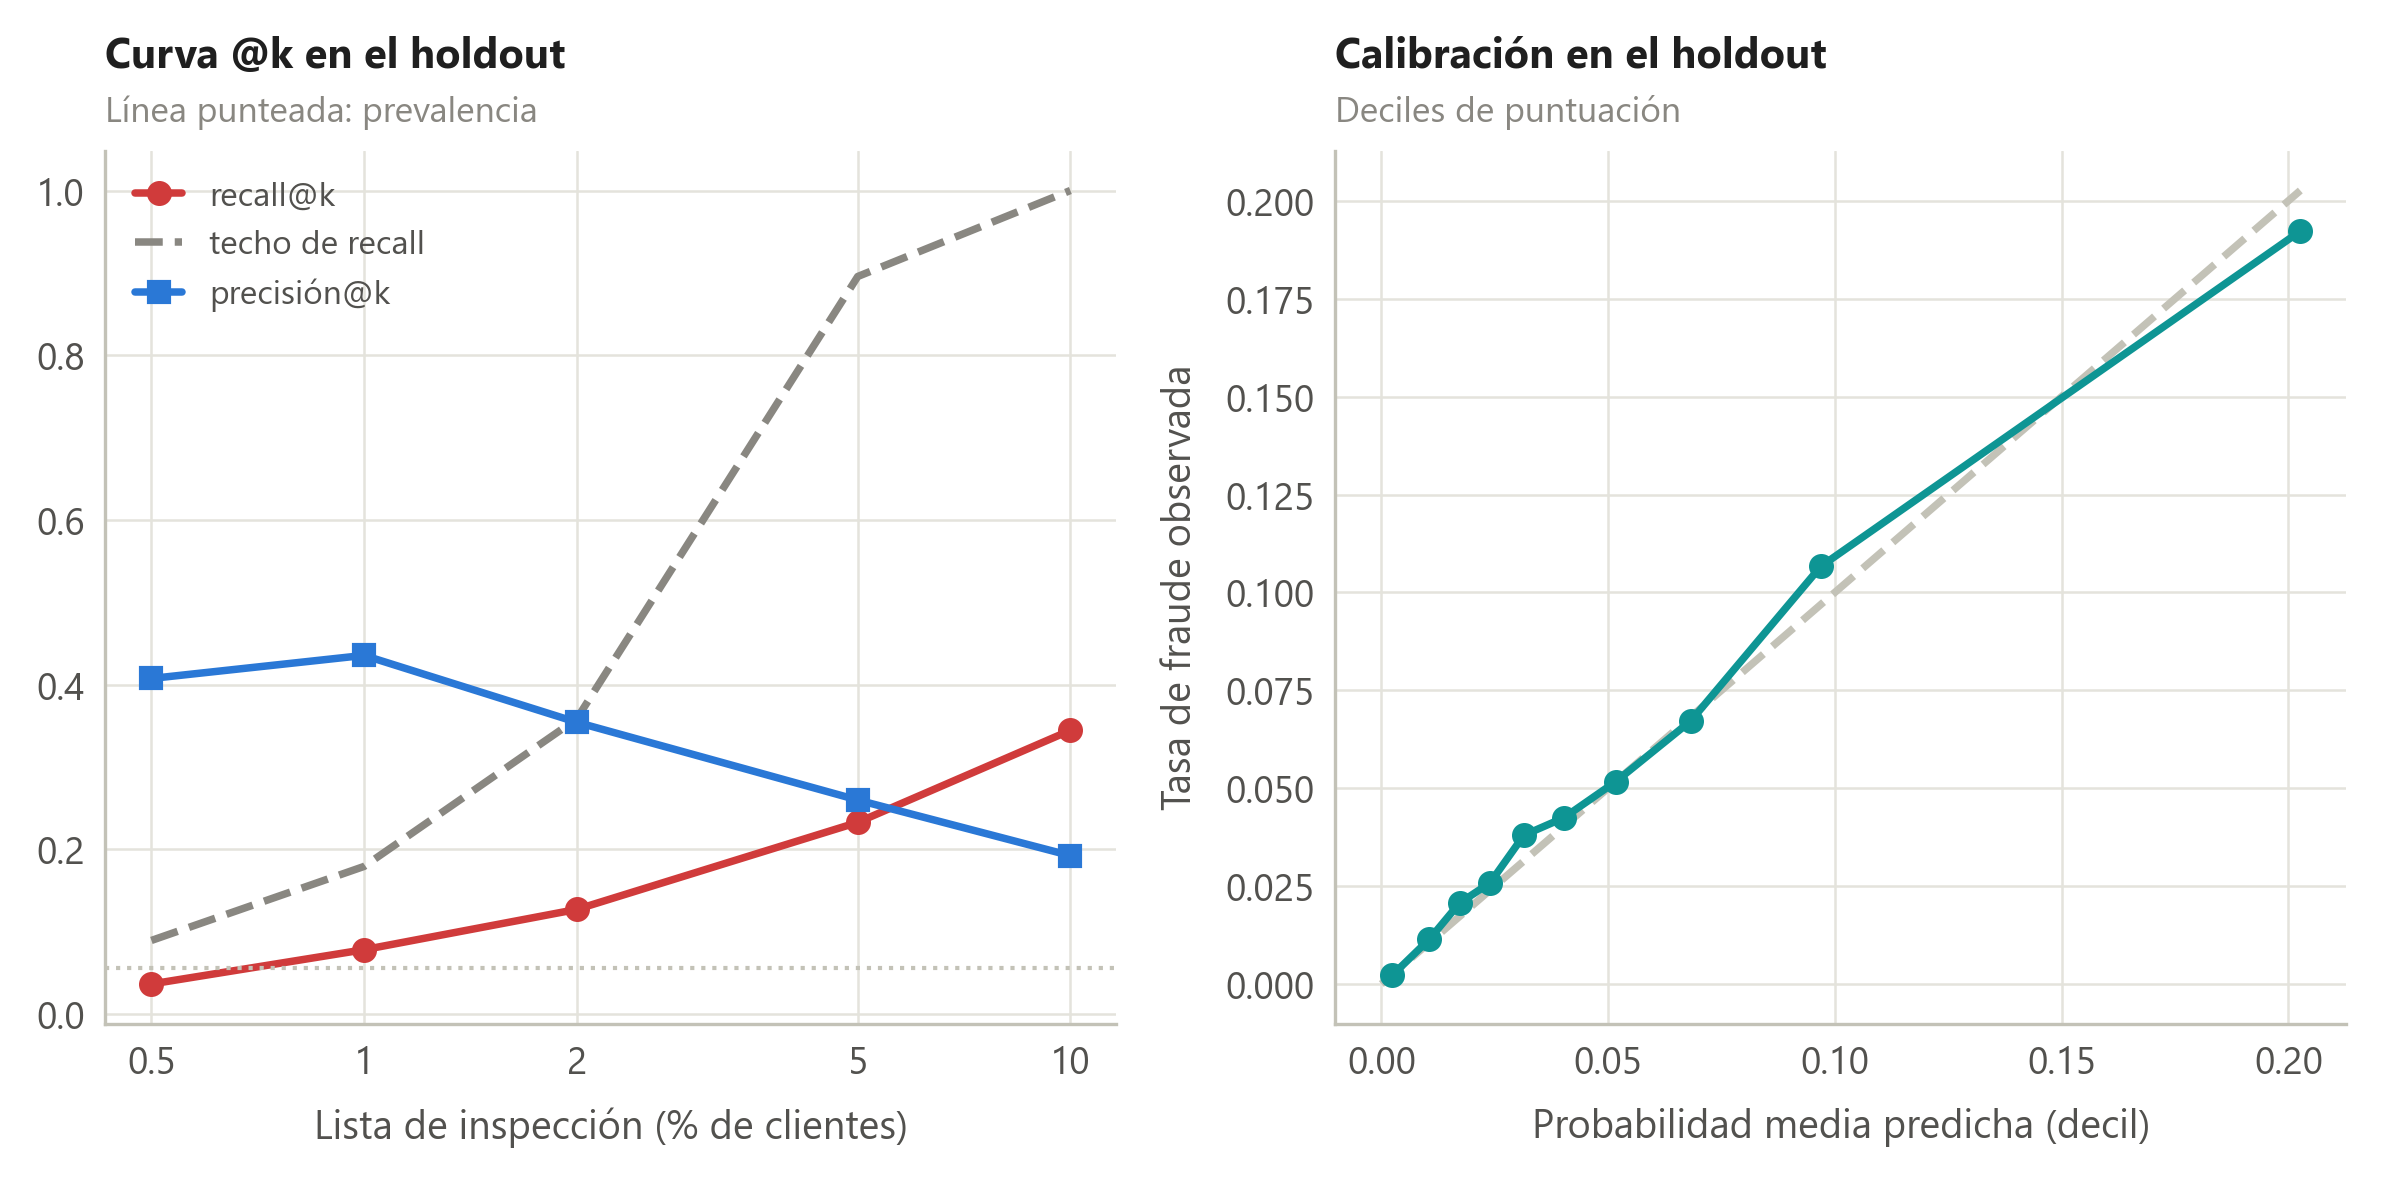
\includegraphics[width=\textwidth]{fig_model_holdout.png}
  \caption{Conjunto de prueba sellado. Izquierda: precisión@$k$, recall@$k$ y techo de recall
    según el tamaño de la lista. Derecha: tasa de fraude observada frente a la probabilidad
    media predicha por decil.}
  \label{fig:holdout}
\end{figure}

\subsubsection{Desempeño por subgrupos}

En los 21.562 clientes del conjunto de prueba sin evento de equipo o de contrato, con una
prevalencia del 2,0\,\%, el modelo obtiene un ROC-AUC de 0,758 y un PR-AUC de 0,086, frente a
0,733 y 0,048 de la línea base de exposición (Tabla~\ref{tab:subgrupos}). La señal se
mantiene donde no hay corte que delatar, como plantea H2. Por quintil de longitud del
historial, el ROC-AUC del modelo en el conjunto de prueba va de 0,676 a 0,798. En el quintil
de historiales más cortos, que solo tiene 54 positivos, la línea base de exposición lo supera
(0,909 frente a 0,798): entre clientes con muy pocas facturas, cuántas tienen sigue
separando a los positivos mejor que su comportamiento. Por distrito, el ROC-AUC va de 0,730
a 0,769.

% Generado por paper/exportar_artefactos.py desde reports/tables/modeling_holdout_por_evento_equipo.csv. No editar a mano.
\begin{table}[htbp]
  \centering
  \small
  \caption{Desempeño en el holdout según el cliente haya tenido o no un evento de equipo o de contrato.}
  \label{tab:subgrupos}
  \begin{threeparttable}
    \begin{tabular}{l S[table-format=5.0] S[table-format=2.1] S[table-format=1.3] S[table-format=1.3] S[table-format=1.3] S[table-format=1.3]}
      \toprule
      {Grupo} & {Clientes} & {Prevalencia (\%)} & {\shortstack{ROC-AUC\\modelo}} & {\shortstack{ROC-AUC\\exposición}} & {\shortstack{PR-AUC\\modelo}} & {\shortstack{PR-AUC\\exposición}} \\
      \midrule
      Sin evento & 21562 & 2.0 & 0.758 & 0.733 & 0.086 & 0.048 \\
      Con evento & 5537 & 19.3 & 0.689 & 0.633 & 0.365 & 0.270 \\
      \bottomrule
    \end{tabular}
    \begin{tablenotes}
      \footnotesize
      \item El grupo sin evento no tiene corte que delatar y da la medida más limpia de la señal de comportamiento.
      \item Fuente: \texttt{reports/tables/modeling\_holdout\_por\_evento\_equipo.csv}.
    \end{tablenotes}
  \end{threeparttable}
\end{table}


\subsubsection{Variables que más pesan}

La familia de tarifa y contador concentra el 31,2\,\% de la contribución SHAP del modelo,
seguida del nivel de consumo (19,6\,\%) y de su dinámica (18,2\,\%)
(Tabla~\ref{tab:shap}). Individualmente, las variables con mayor contribución son la
proporción de facturas con código de contador 207, el percentil 90 del consumo eléctrico, la
región y la pendiente anual del consumo (Figura~\ref{fig:shap}). Los atributos del cliente
aportan el 9,6\,\% y las comparaciones con pares el 7,4\,\%.

% Generado por paper/exportar_artefactos.py desde reports/tables/modeling_importancia_shap.csv. No editar a mano.
\begin{table}[htbp]
  \centering
  \small
  \caption{Participación de cada familia de variables en la media del valor absoluto de SHAP del modelo final.}
  \label{tab:shap}
  \begin{threeparttable}
    \begin{tabular}{l S[table-format=2.0] S[table-format=2.1] l}
      \toprule
      {Familia} & {Variables} & {Participación (\%)} & {Variable con mayor contribución} \\
      \midrule
      Tarifa y contador & 10 & 31.2 & \texttt{inv\_share\_codigo\_contador\_207} \\
      Nivel de consumo & 8 & 19.6 & \texttt{inv\_elec\_log\_cons\_p90} \\
      Dinámica del consumo & 8 & 18.2 & \texttt{inv\_elec\_pendiente\_log\_cons\_anual} \\
      Regularidad de lectura & 9 & 13.9 & \texttt{inv\_share\_estado\_contador\_no\_cero} \\
      Atributos del cliente & 3 & 9.6 & \texttt{cli\_region} \\
      Relativas a pares & 4 & 7.4 & \texttt{rel\_elec\_cons\_vs\_catg} \\
      \bottomrule
    \end{tabular}
    \begin{tablenotes}
      \footnotesize
      \item SHAP calculado sobre 20.000 clientes de \textit{dev}; 42 entradas (38 variables por cliente y 4 relativas a pares).
      \item Fuente: \texttt{reports/tables/modeling\_importancia\_shap.csv}.
    \end{tablenotes}
  \end{threeparttable}
\end{table}


\begin{figure}[htbp]
  \centering
  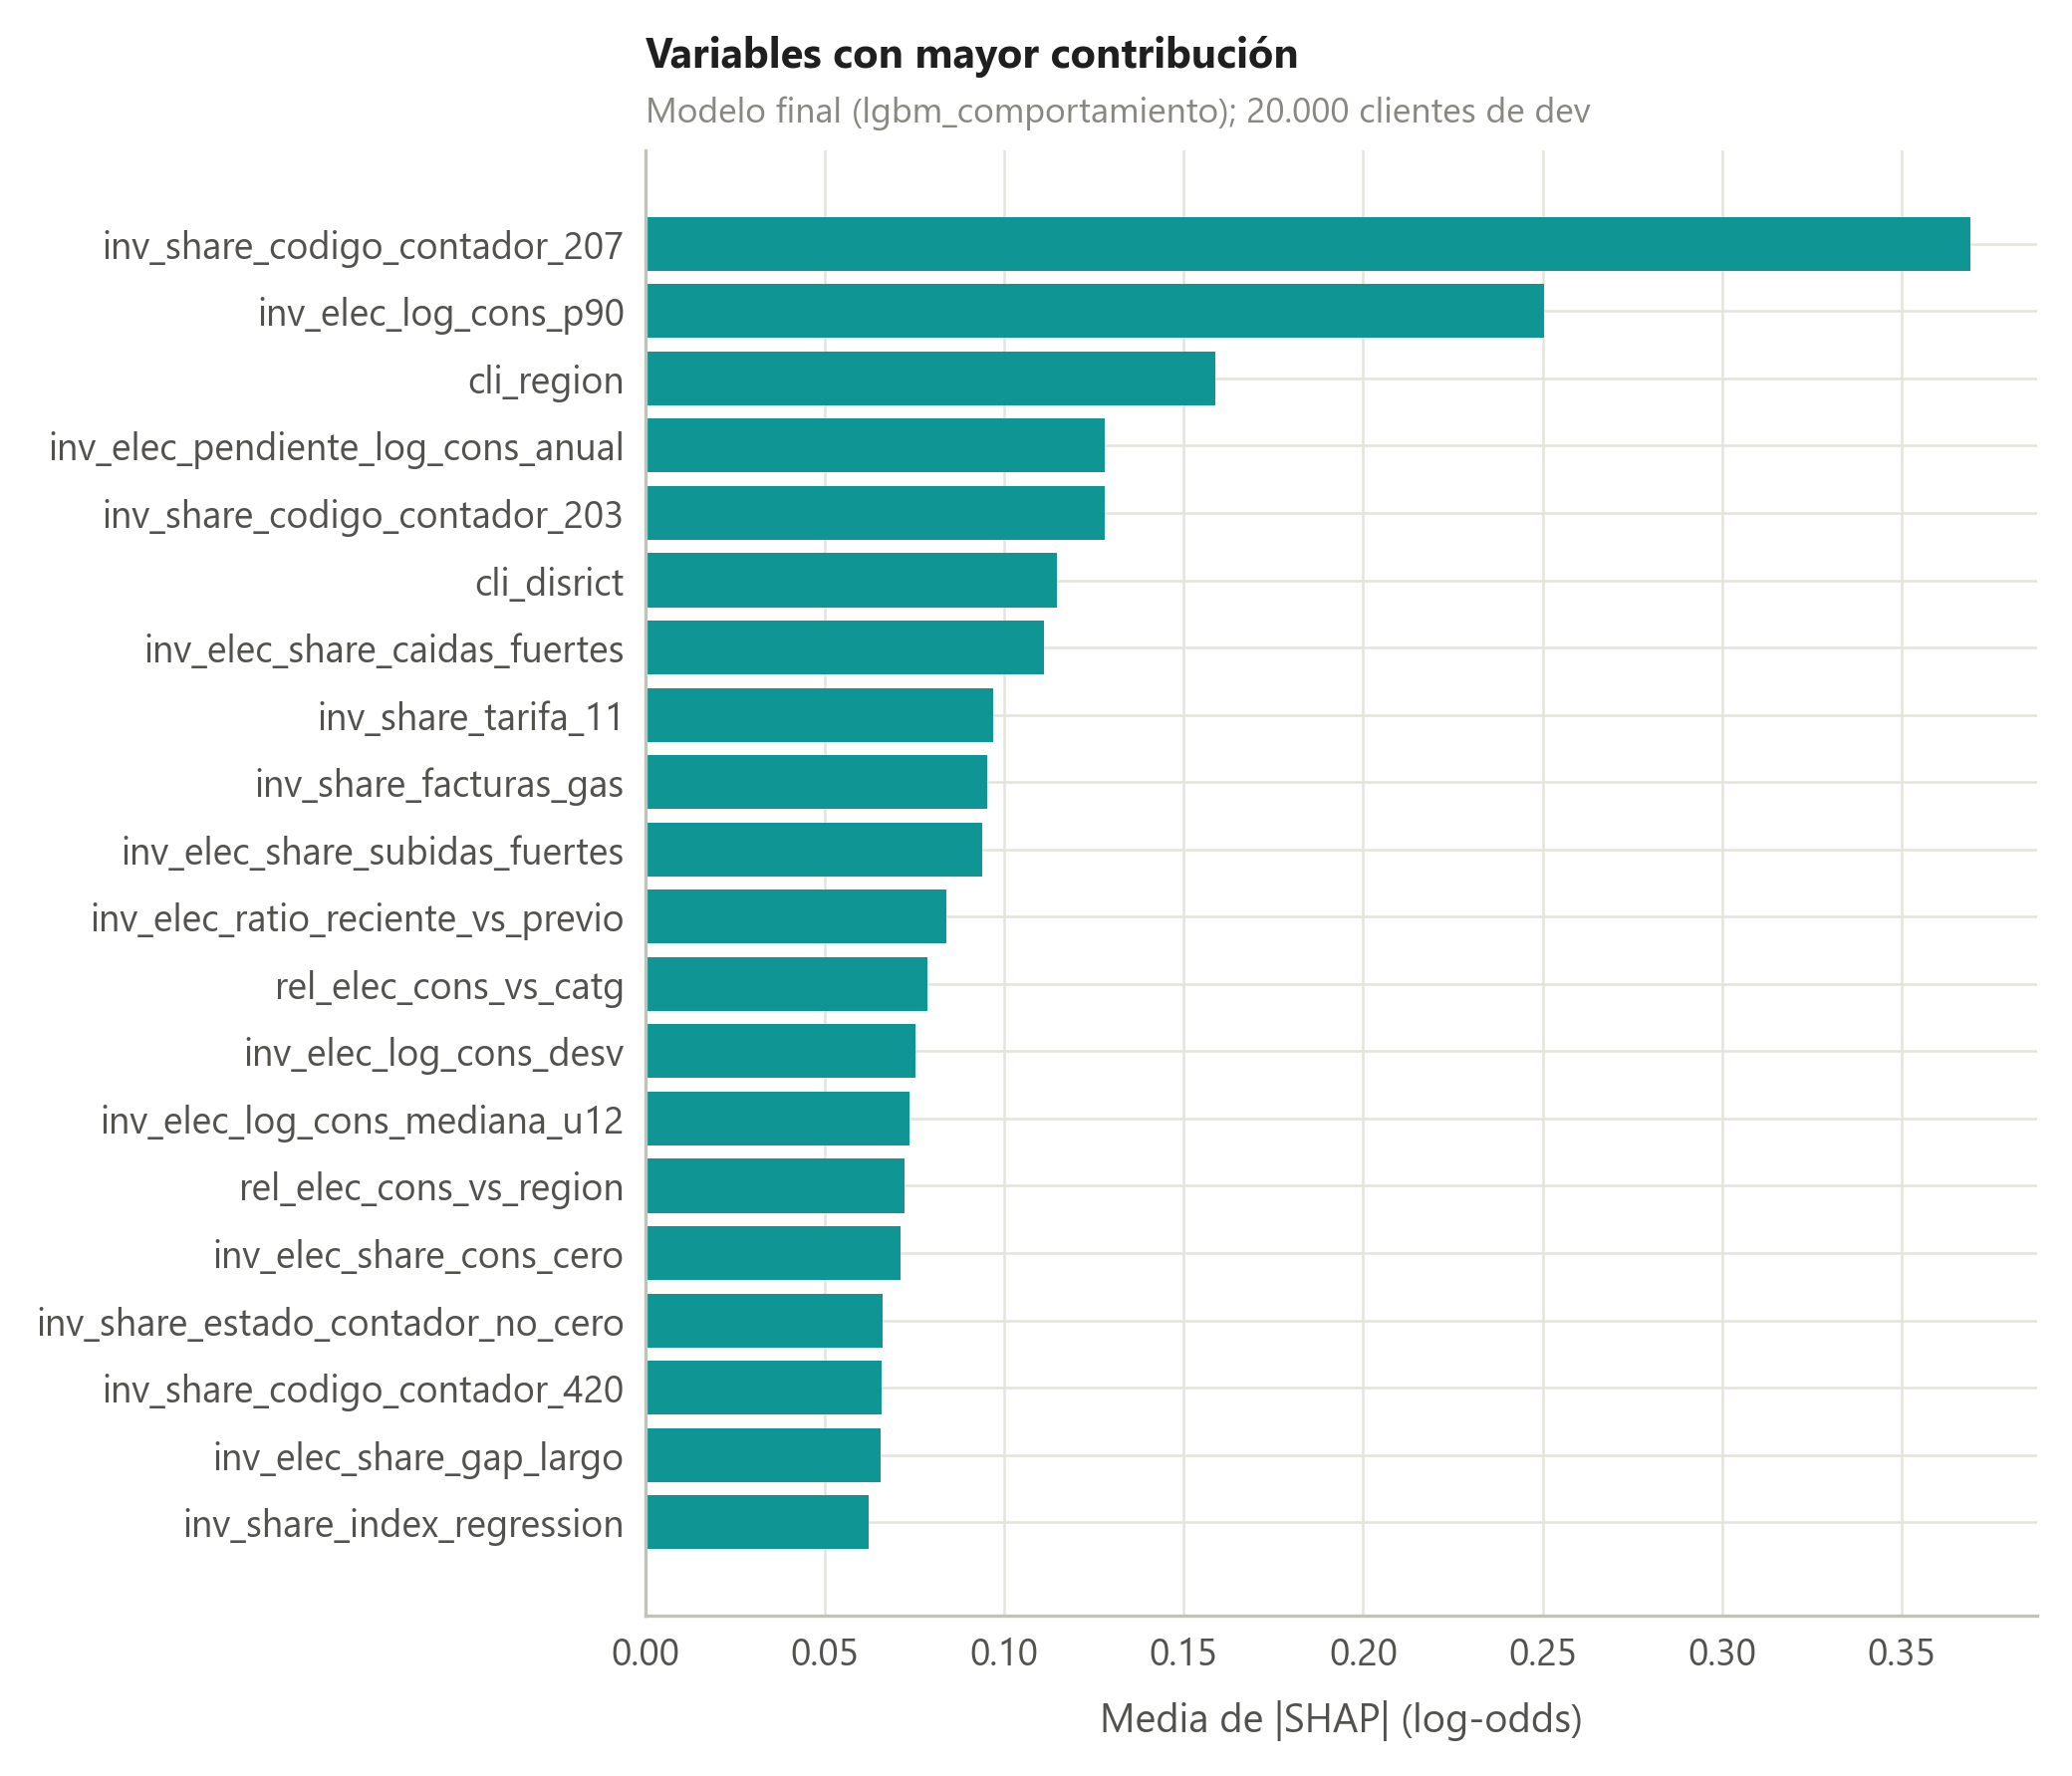
\includegraphics[width=0.8\textwidth]{fig_model_shap_importancia.png}
  \caption{Media del valor absoluto de SHAP de las 20 variables con mayor contribución en el
    modelo final, sobre 20.000 clientes de \textit{dev}.}
  \label{fig:shap}
\end{figure}

\subsection{Respuesta a la pregunta guía}

Las dos hipótesis se sostienen con los datos. H1: la segunda mitad del historial completo
rinde 0,213 más de PR-AUC que la primera, y la censura reduce esa diferencia a 0,032. H2: con
el historial censurado, el modelo encuentra en el 1\,\% superior de la lista el doble de
fraudes que la línea base de exposición y conserva un ROC-AUC de 0,758 entre los clientes sin
eventos. El objetivo general se cumple con un modelo que, sobre clientes que no vio, ordena
con una precisión del 43,5\,\% en la cabeza de la lista frente al 5,58\,\% del azar.
